\documentclass{book}
\usepackage[a4paper,top=2.5cm,bottom=2.5cm,left=2.5cm,right=2.5cm]{geometry}
\usepackage{makeidx}
\usepackage{natbib}
\usepackage{graphicx}
\usepackage{multicol}
\usepackage{float}
\usepackage{listings}
\usepackage{color}
\usepackage{ifthen}
\usepackage[table]{xcolor}
\usepackage{textcomp}
\usepackage{alltt}
\usepackage{ifpdf}
\ifpdf
\usepackage[pdftex,
            pagebackref=true,
            colorlinks=true,
            linkcolor=blue,
            unicode
           ]{hyperref}
\else
\usepackage[ps2pdf,
            pagebackref=true,
            colorlinks=true,
            linkcolor=blue,
            unicode
           ]{hyperref}
\usepackage{pspicture}
\fi
\usepackage[utf8]{inputenc}
\usepackage{mathptmx}
\usepackage[scaled=.90]{helvet}
\usepackage{courier}
\usepackage{sectsty}
\usepackage{amssymb}
\usepackage[titles]{tocloft}
\usepackage{doxygen}
\lstset{language=C++,inputencoding=utf8,basicstyle=\footnotesize,breaklines=true,breakatwhitespace=true,tabsize=4,numbers=left }
\makeindex
\setcounter{tocdepth}{3}
\renewcommand{\footrulewidth}{0.4pt}
\renewcommand{\familydefault}{\sfdefault}
\hfuzz=15pt
\setlength{\emergencystretch}{15pt}
\hbadness=750
\tolerance=750
\begin{document}
\hypersetup{pageanchor=false,citecolor=blue}
\begin{titlepage}
\vspace*{7cm}
\begin{center}
{\Large Thesis Project -\/ Open\-Frameworks Part }\\
\vspace*{1cm}
{\large Generated by Doxygen 1.8.2}\\
\vspace*{0.5cm}
{\small Mon Oct 29 2012 04:23:21}\\
\end{center}
\end{titlepage}
\clearemptydoublepage
\pagenumbering{roman}
\tableofcontents
\clearemptydoublepage
\pagenumbering{arabic}
\hypersetup{pageanchor=true,citecolor=blue}
\chapter{Module Index}
\section{Modules}
Here is a list of all modules\-:\begin{DoxyCompactList}
\item \contentsline{section}{Default Functions}{\pageref{group___open_frame_works}}{}
\item \contentsline{section}{G\-U\-I}{\pageref{group___g_u_i}}{}
\end{DoxyCompactList}

\chapter{Hierarchical Index}
\input{hierarchy}
\chapter{Class Index}
\input{annotated}
\chapter{File Index}
\input{files}
\chapter{Module Documentation}
\hypertarget{group___open_frame_works}{\section{Default Functions}
\label{group___open_frame_works}\index{Default Functions@{Default Functions}}
}


These are the default Functions that are included in an empty Open\-Frame\-Works Project. Main functions to look at are the \hyperlink{group___open_frame_works_gad431db15b6150b965cd52bcba8e16e11}{setup()} and draw() functions.  


\subsection*{Functions}
\begin{DoxyCompactItemize}
\item 
\hypertarget{group___open_frame_works_gad431db15b6150b965cd52bcba8e16e11}{void \hyperlink{group___open_frame_works_gad431db15b6150b965cd52bcba8e16e11}{test\-App\-::setup} ()}\label{group___open_frame_works_gad431db15b6150b965cd52bcba8e16e11}

\begin{DoxyCompactList}\small\item\em Open\-Frameworks First method that is called at the beginning of the program.\-Initialize all Variables Here. \end{DoxyCompactList}\item 
\hypertarget{group___open_frame_works_gafb39d201aec71a295b7609876bf7d0c6}{void {\bfseries test\-App\-::update} ()}\label{group___open_frame_works_gafb39d201aec71a295b7609876bf7d0c6}

\item 
\hypertarget{group___open_frame_works_gaf869cba67b1dab8481f8d0e216d59dcd}{void {\bfseries test\-App\-::draw} ()}\label{group___open_frame_works_gaf869cba67b1dab8481f8d0e216d59dcd}

\item 
\hypertarget{group___open_frame_works_ga904d147c7e532cb92656d5dd4895cd26}{void {\bfseries test\-App\-::key\-Pressed} (int key)}\label{group___open_frame_works_ga904d147c7e532cb92656d5dd4895cd26}

\item 
\hypertarget{group___open_frame_works_ga1116a10088e4932f6d482efe723cd45e}{void {\bfseries test\-App\-::key\-Released} (int key)}\label{group___open_frame_works_ga1116a10088e4932f6d482efe723cd45e}

\item 
\hypertarget{group___open_frame_works_ga33541b19eff9f8285b2487bfc146d58b}{void {\bfseries test\-App\-::mouse\-Moved} (int x, int y)}\label{group___open_frame_works_ga33541b19eff9f8285b2487bfc146d58b}

\item 
\hypertarget{group___open_frame_works_ga075bcc2be16fd8f3eaa9162fb40a0a1f}{void {\bfseries test\-App\-::mouse\-Dragged} (int x, int y, int button)}\label{group___open_frame_works_ga075bcc2be16fd8f3eaa9162fb40a0a1f}

\item 
void \hyperlink{group___open_frame_works_ga3f200702ce91859cac2872a39302679d}{test\-App\-::mouse\-Pressed} (int x, int y, int button)
\begin{DoxyCompactList}\small\item\em Mouse pressed. \end{DoxyCompactList}\item 
\hypertarget{group___open_frame_works_gaa3680ffc782b1e5c451289817f20c9c6}{void {\bfseries test\-App\-::mouse\-Released} (int x, int y, int button)}\label{group___open_frame_works_gaa3680ffc782b1e5c451289817f20c9c6}

\item 
\hypertarget{group___open_frame_works_ga428b7df9c64352d6e7cb234fc297e6c9}{void {\bfseries test\-App\-::window\-Resized} (int w, int h)}\label{group___open_frame_works_ga428b7df9c64352d6e7cb234fc297e6c9}

\end{DoxyCompactItemize}


\subsection{Detailed Description}
These are the default Functions that are included in an empty Open\-Frame\-Works Project. Main functions to look at are the \hyperlink{group___open_frame_works_gad431db15b6150b965cd52bcba8e16e11}{setup()} and draw() functions. 

\subsection{Function Documentation}
\hypertarget{group___open_frame_works_ga3f200702ce91859cac2872a39302679d}{\index{Default Functions@{Default Functions}!mouse\-Pressed@{mouse\-Pressed}}
\index{mouse\-Pressed@{mouse\-Pressed}!Default Functions@{Default Functions}}
\subsubsection[{mouse\-Pressed}]{\setlength{\rightskip}{0pt plus 5cm}void test\-App\-::mouse\-Pressed (
\begin{DoxyParamCaption}
\item[{int}]{x, }
\item[{int}]{y, }
\item[{int}]{button}
\end{DoxyParamCaption}
)}}\label{group___open_frame_works_ga3f200702ce91859cac2872a39302679d}


Mouse pressed. 

\begin{DoxyAuthor}{Author}
Rahul 
\end{DoxyAuthor}
\begin{DoxyDate}{Date}
9/21/2012
\end{DoxyDate}

\begin{DoxyParams}{Parameters}
{\em x} & The x coordinate. \\
\hline
{\em y} & The y coordinate. \\
\hline
{\em button} & The button. \\
\hline
\end{DoxyParams}

\hypertarget{group___g_u_i}{\section{G\-U\-I}
\label{group___g_u_i}\index{G\-U\-I@{G\-U\-I}}
}
\subsection*{Functions}
\begin{DoxyCompactItemize}
\item 
void \hyperlink{group___g_u_i_ga210397e42daad5b2ded2b80598905827}{test\-App\-::setup\-Fonts} ()
\begin{DoxyCompactList}\small\item\em Sets up the fonts These are not used much but can be used during debugging when you want to check which model is selected ..The selected model will appear on upper-\/middle part. \end{DoxyCompactList}\item 
void \hyperlink{group___g_u_i_ga12fd724a9073e84f1367d01f97d222d8}{test\-App\-::draw\-Touch\-Impressions} (vector$<$ string $>$message, bool)
\begin{DoxyCompactList}\small\item\em Draw touch impressions. \end{DoxyCompactList}\end{DoxyCompactItemize}


\subsection{Detailed Description}


\subsection{Function Documentation}
\hypertarget{group___g_u_i_ga12fd724a9073e84f1367d01f97d222d8}{\index{G\-U\-I@{G\-U\-I}!draw\-Touch\-Impressions@{draw\-Touch\-Impressions}}
\index{draw\-Touch\-Impressions@{draw\-Touch\-Impressions}!GUI@{G\-U\-I}}
\subsubsection[{draw\-Touch\-Impressions}]{\setlength{\rightskip}{0pt plus 5cm}void test\-App\-::draw\-Touch\-Impressions (
\begin{DoxyParamCaption}
\item[{vector$<$ string $>$}]{message, }
\item[{bool}]{something\-Selected = {\ttfamily false}}
\end{DoxyParamCaption}
)}}\label{group___g_u_i_ga12fd724a9073e84f1367d01f97d222d8}


Draw touch impressions. 

\begin{DoxyAuthor}{Author}
Rahul 
\end{DoxyAuthor}
\begin{DoxyDate}{Date}
10/28/2012
\end{DoxyDate}

\begin{DoxyParams}{Parameters}
{\em message} & The Split components of the message \\
\hline
{\em something\-Selected} & (optional) Is something selected ?. \\
\hline
\end{DoxyParams}
\hypertarget{group___g_u_i_ga210397e42daad5b2ded2b80598905827}{\index{G\-U\-I@{G\-U\-I}!setup\-Fonts@{setup\-Fonts}}
\index{setup\-Fonts@{setup\-Fonts}!GUI@{G\-U\-I}}
\subsubsection[{setup\-Fonts}]{\setlength{\rightskip}{0pt plus 5cm}void test\-App\-::setup\-Fonts (
\begin{DoxyParamCaption}
{}
\end{DoxyParamCaption}
)}}\label{group___g_u_i_ga210397e42daad5b2ded2b80598905827}


Sets up the fonts These are not used much but can be used during debugging when you want to check which model is selected ..The selected model will appear on upper-\/middle part. 

load our type 
\chapter{Class Documentation}
\input{class_calculations}
\input{class_g_u_i_stuff}
\input{class_models}
\input{class_note_information}
\input{class_p_o_is}
\hypertarget{classtest_app}{\section{test\-App Class Reference}
\label{classtest_app}\index{test\-App@{test\-App}}
}


Test application.  




{\ttfamily \#include $<$test\-App.\-h$>$}

Inheritance diagram for test\-App\-:\begin{figure}[H]
\begin{center}
\leavevmode
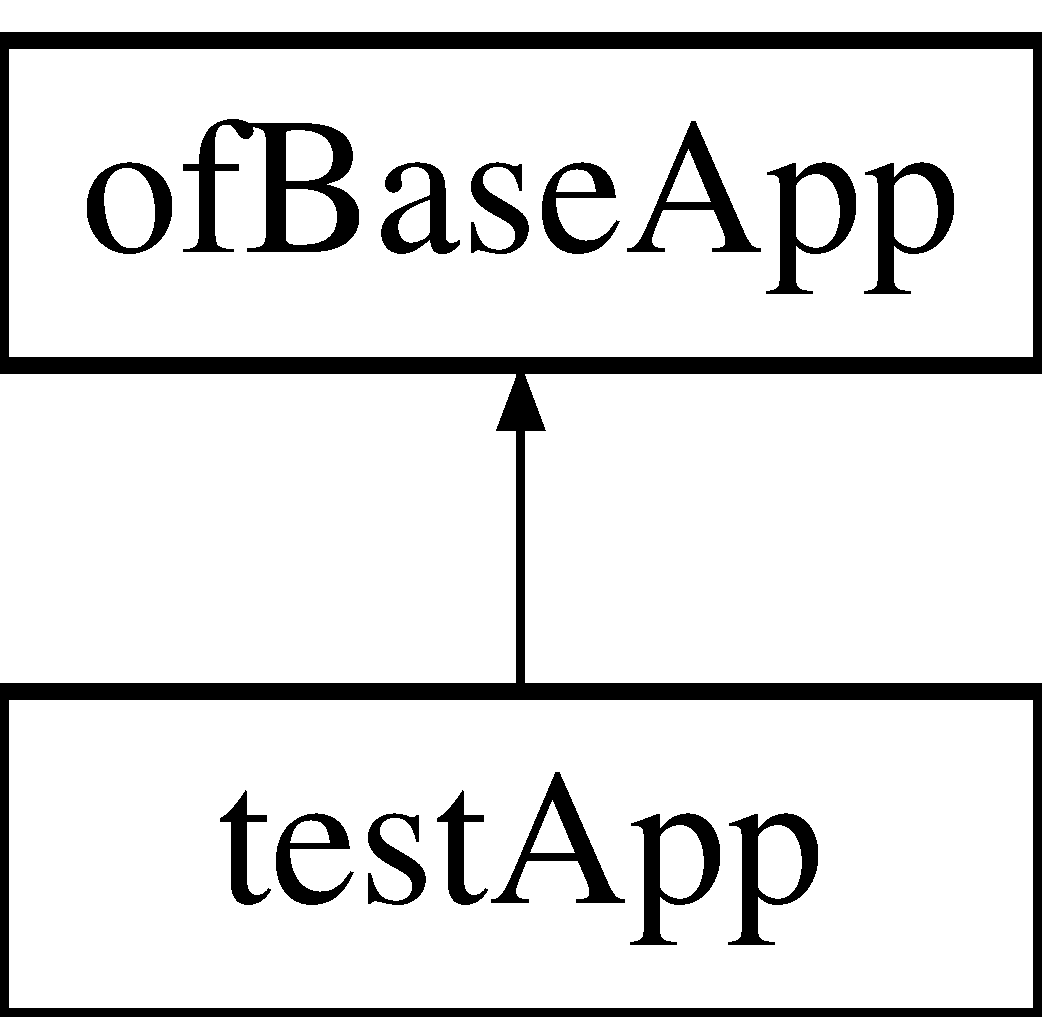
\includegraphics[height=2.000000cm]{classtest_app}
\end{center}
\end{figure}
\subsection*{Public Member Functions}
\begin{DoxyCompactItemize}
\item 
\hypertarget{group___open_frame_works_gad431db15b6150b965cd52bcba8e16e11}{void \hyperlink{group___open_frame_works_gad431db15b6150b965cd52bcba8e16e11}{setup} ()}\label{group___open_frame_works_gad431db15b6150b965cd52bcba8e16e11}

\begin{DoxyCompactList}\small\item\em Open\-Frameworks First method that is called at the beginning of the program.\-Initialize all Variables Here. \end{DoxyCompactList}\item 
\hypertarget{group___open_frame_works_gafb39d201aec71a295b7609876bf7d0c6}{void {\bfseries update} ()}\label{group___open_frame_works_gafb39d201aec71a295b7609876bf7d0c6}

\item 
\hypertarget{group___open_frame_works_gaf869cba67b1dab8481f8d0e216d59dcd}{void {\bfseries draw} ()}\label{group___open_frame_works_gaf869cba67b1dab8481f8d0e216d59dcd}

\item 
\hypertarget{group___open_frame_works_ga904d147c7e532cb92656d5dd4895cd26}{void {\bfseries key\-Pressed} (int key)}\label{group___open_frame_works_ga904d147c7e532cb92656d5dd4895cd26}

\item 
\hypertarget{group___open_frame_works_ga1116a10088e4932f6d482efe723cd45e}{void {\bfseries key\-Released} (int key)}\label{group___open_frame_works_ga1116a10088e4932f6d482efe723cd45e}

\item 
\hypertarget{group___open_frame_works_ga33541b19eff9f8285b2487bfc146d58b}{void {\bfseries mouse\-Moved} (int x, int y)}\label{group___open_frame_works_ga33541b19eff9f8285b2487bfc146d58b}

\item 
\hypertarget{group___open_frame_works_ga075bcc2be16fd8f3eaa9162fb40a0a1f}{void {\bfseries mouse\-Dragged} (int x, int y, int button)}\label{group___open_frame_works_ga075bcc2be16fd8f3eaa9162fb40a0a1f}

\item 
void \hyperlink{group___open_frame_works_ga3f200702ce91859cac2872a39302679d}{mouse\-Pressed} (int x, int y, int button)
\begin{DoxyCompactList}\small\item\em Mouse pressed. \end{DoxyCompactList}\item 
\hypertarget{group___open_frame_works_gaa3680ffc782b1e5c451289817f20c9c6}{void {\bfseries mouse\-Released} (int x, int y, int button)}\label{group___open_frame_works_gaa3680ffc782b1e5c451289817f20c9c6}

\item 
\hypertarget{group___open_frame_works_ga428b7df9c64352d6e7cb234fc297e6c9}{void {\bfseries window\-Resized} (int w, int h)}\label{group___open_frame_works_ga428b7df9c64352d6e7cb234fc297e6c9}

\item 
void \hyperlink{classtest_app_a853bbabdab3e7d2f207bb5a2028990bd}{Update\-Tracking} ()
\begin{DoxyCompactList}\small\item\em Updates the tracking received from the Vuzix i-\/\-Wear Tracker. \end{DoxyCompactList}\item 
void \hyperlink{classtest_app_a6a4db7a6a914fc4899763fc94bfca4b7}{setup\-Tracker} ()
\begin{DoxyCompactList}\small\item\em Sets up the Vuzix i\-Wear Tracker. \end{DoxyCompactList}\item 
void \hyperlink{classtest_app_aa1d58aa9130d8d7526eb407f13f7a833}{add\-Objectto\-Scene} (string)
\item 
\hypertarget{classtest_app_a689f3b0cf0b38217152da7f5ce0d609f}{of\-Color {\bfseries Returncolor} (string)}\label{classtest_app_a689f3b0cf0b38217152da7f5ce0d609f}

\item 
void \hyperlink{classtest_app_a34646de458b0af33bc02457c9b8583df}{draw\-Augmented\-Plane} (float, float, of\-Color, of\-Color, int, string, string)
\begin{DoxyCompactList}\small\item\em Takes information from Handheld Phone and draws augmented plane in the A\-R view. \end{DoxyCompactList}\item 
void \hyperlink{classtest_app_ae9ee24f0c2bec5965519deef1a14da16}{translate\-\_\-3\-D\-\_\-\-Model} (string)
\begin{DoxyCompactList}\small\item\em Translate 3 d model.ip\%. \end{DoxyCompactList}\item 
void \hyperlink{group___g_u_i_ga210397e42daad5b2ded2b80598905827}{setup\-Fonts} ()
\begin{DoxyCompactList}\small\item\em Sets up the fonts These are not used much but can be used during debugging when you want to check which model is selected ..The selected model will appear on upper-\/middle part. \end{DoxyCompactList}\item 
void \hyperlink{group___g_u_i_ga12fd724a9073e84f1367d01f97d222d8}{draw\-Touch\-Impressions} (vector$<$ string $>$message, bool)
\begin{DoxyCompactList}\small\item\em Draw touch impressions. \end{DoxyCompactList}\item 
\hypertarget{classtest_app_aae96728967b563fab5b52350915829b7}{void {\bfseries setup\-Crosshair} ()}\label{classtest_app_aae96728967b563fab5b52350915829b7}

\item 
\hypertarget{classtest_app_a4f0adc57489b13878194958d0f2da032}{void {\bfseries update\-Model\-Positions} ()}\label{classtest_app_a4f0adc57489b13878194958d0f2da032}

\item 
\hypertarget{classtest_app_a9d57148d51d852b0fe1051ee150f0fc0}{void {\bfseries draw\-Crosshair} ()}\label{classtest_app_a9d57148d51d852b0fe1051ee150f0fc0}

\item 
\hypertarget{classtest_app_a9388efd101d9850bdf41ed036861e369}{string {\bfseries Receive\-\_\-\-Message} ()}\label{classtest_app_a9388efd101d9850bdf41ed036861e369}

\item 
void \hyperlink{classtest_app_a8afafb31eb516994348caaf54bdea6bb}{translate\-Model} (vector$<$ string $>$)
\item 
\hypertarget{classtest_app_aff620776a9cf806d8555de9a501fdcee}{void {\bfseries store\-Finger\-Position} (vector$<$ string $>$)}\label{classtest_app_aff620776a9cf806d8555de9a501fdcee}

\item 
\hypertarget{classtest_app_a5631a4b034f1558b451fed3868480222}{void {\bfseries Check\-\_\-if\-\_\-\-Finger\-\_\-\-Intersects\-\_\-3\-D\-Model} (vector$<$ string $>$)}\label{classtest_app_a5631a4b034f1558b451fed3868480222}

\item 
void \hyperlink{classtest_app_ac374af2c9d11d72f27d79e16f3902b95}{reset\-Model\-Variables} ()
\item 
\hypertarget{classtest_app_a2397b9317004e36fb25ca77bb7f99d50}{int {\bfseries Check\-\_\-for\-\_\-\-Finger\-\_\-\-Intersections} ()}\label{classtest_app_a2397b9317004e36fb25ca77bb7f99d50}

\item 
void \hyperlink{classtest_app_af4304932dc358f431608e54b243f74e5}{convert\-Phoneto\-Screen\-Coordinates} (string raw\-Touch\-Points)
\begin{DoxyCompactList}\small\item\em Convert phone to screen coordinates. \end{DoxyCompactList}\item 
\hypertarget{classtest_app_ae813833c1d2e4917d75984d1828f0c30}{void {\bfseries temp\-\_\-calculate\-Maxand\-Min} ()}\label{classtest_app_ae813833c1d2e4917d75984d1828f0c30}

\item 
\hypertarget{classtest_app_acff4b4d2d795806c8586f83602457ed7}{int {\bfseries Check\-\_\-for\-\_\-crosshair\-\_\-model\-\_\-intersection} ()}\label{classtest_app_acff4b4d2d795806c8586f83602457ed7}

\end{DoxyCompactItemize}
\begin{Indent}{\bf U\-D\-P\-Receive}\par
{\em This function will receive the U\-D\-P Packets and check whether the command sent from the Android Phone includes information about adding a Notes Pane. If a note is added,then the message will be received in the format \char`\"{}note,\-Latitude\-\_\-of\-\_\-note,\-Longitude\-\_\-of\-\_\-note,\-Note Heading,\-Note Text\char`\"{}

\begin{DoxyAuthor}{Author}
Rahul 
\end{DoxyAuthor}
\begin{DoxyDate}{Date}
10/28/2012 
\end{DoxyDate}
}\begin{DoxyCompactItemize}
\item 
\hypertarget{classtest_app_ae18e12d5025a2167ebd63ca019468cc0}{void {\bfseries U\-D\-P\-Receive} ()}\label{classtest_app_ae18e12d5025a2167ebd63ca019468cc0}

\end{DoxyCompactItemize}
\end{Indent}
\begin{Indent}{\bf G\-U\-I stuff ..}\par
{\em G\-U\-I\-Functions

These Functions can be easily replaced as Open\-Frame\-Works already has functions for the same ,but I am keeping them here for now .. }\begin{DoxyCompactItemize}
\item 
void \hyperlink{classtest_app_aa2fcbae31171ba366d4c0fcaf44149f4}{draw\-Axes} ()
\begin{DoxyCompactList}\small\item\em Draw axes. \end{DoxyCompactList}\item 
\hypertarget{classtest_app_a47747729f6d0d84c36ef0ec9fca01303}{void {\bfseries draw\-Plane} ()}\label{classtest_app_a47747729f6d0d84c36ef0ec9fca01303}

\item 
void \hyperlink{classtest_app_a16036c3aa23c1747e315a3e18105cf45}{draw\-Touches} (string udp\-Message)
\begin{DoxyCompactList}\small\item\em If the Handheld is being used a controller,This function will take the touch information and draw it on the A\-R view. \end{DoxyCompactList}\end{DoxyCompactItemize}
\end{Indent}
\subsection*{Public Attributes}
\begin{DoxyCompactItemize}
\item 
\hypertarget{classtest_app_a9bcefa3afb830941451f72174a36b722}{of\-True\-Type\-Font \hyperlink{classtest_app_a9bcefa3afb830941451f72174a36b722}{mono}}\label{classtest_app_a9bcefa3afb830941451f72174a36b722}

\begin{DoxyCompactList}\small\item\em The Font Variable,Will store the fonts used for debugging... \end{DoxyCompactList}\item 
\hypertarget{classtest_app_afc42ad25d37b1292d27d783380249424}{of\-True\-Type\-Font \hyperlink{classtest_app_afc42ad25d37b1292d27d783380249424}{monosm}}\label{classtest_app_afc42ad25d37b1292d27d783380249424}

\begin{DoxyCompactList}\small\item\em The monosm. \end{DoxyCompactList}\item 
\hypertarget{classtest_app_a9ed611377cd46f5148a3a3d538e96484}{int {\bfseries window\-Width}}\label{classtest_app_a9ed611377cd46f5148a3a3d538e96484}

\item 
int \hyperlink{classtest_app_a31efaa85f8a900bb659a537d56c73e03}{window\-Height}
\begin{DoxyCompactList}\small\item\em Gets the width and height of the window. \end{DoxyCompactList}\item 
\hypertarget{classtest_app_a0db6626782419f4340a3186e51788074}{int {\bfseries gesture\-Type}}\label{classtest_app_a0db6626782419f4340a3186e51788074}

\item 
\hypertarget{classtest_app_a75ac9dc8ee1df4ae07b93a9b74131924}{bool {\bfseries last\-\_\-gesture\-\_\-selected}}\label{classtest_app_a75ac9dc8ee1df4ae07b93a9b74131924}

\item 
\hypertarget{classtest_app_aa2d09c9954dc56b2aaacc99d05948885}{bool {\bfseries begin\-Selection}}\label{classtest_app_aa2d09c9954dc56b2aaacc99d05948885}

\item 
\hypertarget{classtest_app_afea17ef4df91c9cd446cd99f9b8e2ddb}{float {\bfseries scalex\-Position}}\label{classtest_app_afea17ef4df91c9cd446cd99f9b8e2ddb}

\item 
\hypertarget{classtest_app_a9e86476934494e86dd955d5888333795}{float {\bfseries scaley\-Position}}\label{classtest_app_a9e86476934494e86dd955d5888333795}

\item 
\hypertarget{classtest_app_a862943de1cd06690befd3740f6711762}{float {\bfseries scale\-Factor}}\label{classtest_app_a862943de1cd06690befd3740f6711762}

\item 
\hypertarget{classtest_app_a4764bd1bead24898cc3858707ee14ed9}{vector$<$ float $>$ {\bfseries converted\-Touch\-Points}}\label{classtest_app_a4764bd1bead24898cc3858707ee14ed9}

\item 
\hypertarget{classtest_app_a0d9a8da39f01ebe05efbaef7dc2744ea}{vector$<$ float $>$ {\bfseries Crosshair\-\_\-coords}}\label{classtest_app_a0d9a8da39f01ebe05efbaef7dc2744ea}

\item 
\hypertarget{classtest_app_abd2b58403a31a721e2201c3012d3b4e3}{int {\bfseries crosshair\-\_\-selected}}\label{classtest_app_abd2b58403a31a721e2201c3012d3b4e3}

\item 
\hypertarget{classtest_app_a4930c7e7ecb7783261349fd2f2e22f8b}{int \hyperlink{classtest_app_a4930c7e7ecb7783261349fd2f2e22f8b}{Android\-Phone\-Res\-Width}}\label{classtest_app_a4930c7e7ecb7783261349fd2f2e22f8b}

\begin{DoxyCompactList}\small\item\em Width of the Android Phone's Screen Resolution. \end{DoxyCompactList}\item 
\hypertarget{classtest_app_a9389fab48c7bd5896f26d494fa238535}{int \hyperlink{classtest_app_a9389fab48c7bd5896f26d494fa238535}{Android\-Phone\-Res\-Height}}\label{classtest_app_a9389fab48c7bd5896f26d494fa238535}

\begin{DoxyCompactList}\small\item\em Height of the Android Phone's Screen Resolution. \end{DoxyCompactList}\end{DoxyCompactItemize}
\subsection*{U\-D\-P Connection Variables}
\label{_amgrpae40690cdbe7726518333e6d2c1b11b8}%
These Variables will be used to setup the U\-D\-P connections \begin{DoxyCompactItemize}
\item 
\hypertarget{classtest_app_a30c39505591fda7ed8ef4d8c4f0128fd}{ofx\-U\-D\-P\-Manager \hyperlink{classtest_app_a30c39505591fda7ed8ef4d8c4f0128fd}{udp\-Connection}}\label{classtest_app_a30c39505591fda7ed8ef4d8c4f0128fd}

\begin{DoxyCompactList}\small\item\em The U\-D\-P connection. \end{DoxyCompactList}\item 
\hypertarget{classtest_app_a35f96e427475843d44539f125ca454cd}{ofx\-U\-D\-P\-Manager \hyperlink{classtest_app_a35f96e427475843d44539f125ca454cd}{udp\-Send\-Connection}}\label{classtest_app_a35f96e427475843d44539f125ca454cd}

\begin{DoxyCompactList}\small\item\em The U\-D\-P send connection. \end{DoxyCompactList}\item 
\hypertarget{classtest_app_a630d5b8b53aee0c07dc79db616f4eb48}{ofx\-U\-D\-P\-Manager \hyperlink{classtest_app_a630d5b8b53aee0c07dc79db616f4eb48}{udp\-Receive\-Connection}}\label{classtest_app_a630d5b8b53aee0c07dc79db616f4eb48}

\begin{DoxyCompactList}\small\item\em The U\-D\-P receive connection. \end{DoxyCompactList}\item 
\hypertarget{classtest_app_a0d5c58a4c1ebdb291618b34d5237f77b}{void \hyperlink{classtest_app_a0d5c58a4c1ebdb291618b34d5237f77b}{setup\-U\-D\-P\-Connections} ()}\label{classtest_app_a0d5c58a4c1ebdb291618b34d5237f77b}

\begin{DoxyCompactList}\small\item\em Sets up the Connections and Opens the ports. \end{DoxyCompactList}\end{DoxyCompactItemize}
\subsection*{X\-M\-L Stuff}
\label{_amgrp30ed6d911a1420be854691672138b449}%
Takes care of loading the \hyperlink{class_models}{Models} from the X\-M\-L file,Storage,Displaying and Checking if the fingers touch the Model. \begin{DoxyCompactItemize}
\item 
\hypertarget{classtest_app_aa20473a935d49170d16dd7da21124056}{ofx\-Xml\-Settings {\bfseries Models\-File}}\label{classtest_app_aa20473a935d49170d16dd7da21124056}

\item 
\hypertarget{classtest_app_a1bfb9be4aa89d5b89983defa2d235113}{vector$<$ \hyperlink{class_models}{Models} $>$ {\bfseries Models\-List}}\label{classtest_app_a1bfb9be4aa89d5b89983defa2d235113}

\item 
\hypertarget{classtest_app_a307def5df81c899db2107fa85ef6a081}{void \hyperlink{classtest_app_a307def5df81c899db2107fa85ef6a081}{load\-Modelsfrom\-X\-M\-L} ()}\label{classtest_app_a307def5df81c899db2107fa85ef6a081}

\begin{DoxyCompactList}\small\item\em Load \hyperlink{class_models}{Models} from the X\-M\-L file. \end{DoxyCompactList}\item 
\hypertarget{classtest_app_aca7cf2d8efb6d7ccecadf86bb97afc2b}{void \hyperlink{classtest_app_aca7cf2d8efb6d7ccecadf86bb97afc2b}{draw\-Models\-X\-M\-L} ()}\label{classtest_app_aca7cf2d8efb6d7ccecadf86bb97afc2b}

\begin{DoxyCompactList}\small\item\em Draws the models Loaded from the X\-M\-L file (Default\-:data/\-Models.\-xml). \end{DoxyCompactList}\end{DoxyCompactItemize}


\subsection{Detailed Description}
Test application. 

\begin{DoxyAuthor}{Author}
Rahul 
\end{DoxyAuthor}
\begin{DoxyDate}{Date}
9/21/2012 
\end{DoxyDate}


\subsection{Member Function Documentation}
\hypertarget{classtest_app_aa1d58aa9130d8d7526eb407f13f7a833}{\index{test\-App@{test\-App}!add\-Objectto\-Scene@{add\-Objectto\-Scene}}
\index{add\-Objectto\-Scene@{add\-Objectto\-Scene}!testApp@{test\-App}}
\subsubsection[{add\-Objectto\-Scene}]{\setlength{\rightskip}{0pt plus 5cm}void test\-App\-::add\-Objectto\-Scene (
\begin{DoxyParamCaption}
\item[{string}]{message}
\end{DoxyParamCaption}
)}}\label{classtest_app_aa1d58aa9130d8d7526eb407f13f7a833}
\hypertarget{classtest_app_af4304932dc358f431608e54b243f74e5}{\index{test\-App@{test\-App}!convert\-Phoneto\-Screen\-Coordinates@{convert\-Phoneto\-Screen\-Coordinates}}
\index{convert\-Phoneto\-Screen\-Coordinates@{convert\-Phoneto\-Screen\-Coordinates}!testApp@{test\-App}}
\subsubsection[{convert\-Phoneto\-Screen\-Coordinates}]{\setlength{\rightskip}{0pt plus 5cm}void test\-App\-::convert\-Phoneto\-Screen\-Coordinates (
\begin{DoxyParamCaption}
\item[{string}]{raw\-Touch\-Points}
\end{DoxyParamCaption}
)}}\label{classtest_app_af4304932dc358f431608e54b243f74e5}


Convert phone to screen coordinates. 


\begin{DoxyParams}{Parameters}
{\em raw\-Touch\-Points} & The raw touch points. \\
\hline
\end{DoxyParams}
\hypertarget{classtest_app_a34646de458b0af33bc02457c9b8583df}{\index{test\-App@{test\-App}!draw\-Augmented\-Plane@{draw\-Augmented\-Plane}}
\index{draw\-Augmented\-Plane@{draw\-Augmented\-Plane}!testApp@{test\-App}}
\subsubsection[{draw\-Augmented\-Plane}]{\setlength{\rightskip}{0pt plus 5cm}void test\-App\-::draw\-Augmented\-Plane (
\begin{DoxyParamCaption}
\item[{float}]{x\-Position, }
\item[{float}]{y\-Position, }
\item[{of\-Color}]{text\-Color, }
\item[{of\-Color}]{bg\-Color, }
\item[{int}]{i, }
\item[{string}]{note\-\_\-heading, }
\item[{string}]{note\-\_\-text}
\end{DoxyParamCaption}
)}}\label{classtest_app_a34646de458b0af33bc02457c9b8583df}


Takes information from Handheld Phone and draws augmented plane in the A\-R view. 

\begin{DoxyAuthor}{Author}
Rahul 
\end{DoxyAuthor}
\begin{DoxyDate}{Date}
9/28/2012
\end{DoxyDate}

\begin{DoxyParams}{Parameters}
{\em x\-Position} & The x-\/position. \\
\hline
{\em y\-Position} & The y-\/position. \\
\hline
{\em text\-Color} & The color of the text written on the plane. \\
\hline
{\em bg\-Color} & The background color of the plane. \\
\hline
{\em i} & Index,Which Plane is being changed. \\
\hline
{\em note\-\_\-heading} & The note heading. \\
\hline
{\em note\-\_\-text} & The note text. \\
\hline
\end{DoxyParams}
\hypertarget{classtest_app_aa2fcbae31171ba366d4c0fcaf44149f4}{\index{test\-App@{test\-App}!draw\-Axes@{draw\-Axes}}
\index{draw\-Axes@{draw\-Axes}!testApp@{test\-App}}
\subsubsection[{draw\-Axes}]{\setlength{\rightskip}{0pt plus 5cm}void test\-App\-::draw\-Axes (
\begin{DoxyParamCaption}
{}
\end{DoxyParamCaption}
)}}\label{classtest_app_aa2fcbae31171ba366d4c0fcaf44149f4}


Draw axes. 

\begin{DoxyAuthor}{Author}
Rahul 
\end{DoxyAuthor}
\begin{DoxyDate}{Date}
10/28/2012 
\end{DoxyDate}
\hypertarget{classtest_app_a16036c3aa23c1747e315a3e18105cf45}{\index{test\-App@{test\-App}!draw\-Touches@{draw\-Touches}}
\index{draw\-Touches@{draw\-Touches}!testApp@{test\-App}}
\subsubsection[{draw\-Touches}]{\setlength{\rightskip}{0pt plus 5cm}void test\-App\-::draw\-Touches (
\begin{DoxyParamCaption}
\item[{string}]{udp\-Message}
\end{DoxyParamCaption}
)}}\label{classtest_app_a16036c3aa23c1747e315a3e18105cf45}


If the Handheld is being used a controller,This function will take the touch information and draw it on the A\-R view. 

\begin{DoxyAuthor}{Author}
Rahul 
\end{DoxyAuthor}
\begin{DoxyDate}{Date}
9/28/2012
\end{DoxyDate}

\begin{DoxyParams}{Parameters}
{\em udp\-Message} & The Message received though U\-D\-P .. \\
\hline
\end{DoxyParams}
\hypertarget{classtest_app_ac374af2c9d11d72f27d79e16f3902b95}{\index{test\-App@{test\-App}!reset\-Model\-Variables@{reset\-Model\-Variables}}
\index{reset\-Model\-Variables@{reset\-Model\-Variables}!testApp@{test\-App}}
\subsubsection[{reset\-Model\-Variables}]{\setlength{\rightskip}{0pt plus 5cm}void test\-App\-::reset\-Model\-Variables (
\begin{DoxyParamCaption}
{}
\end{DoxyParamCaption}
)}}\label{classtest_app_ac374af2c9d11d72f27d79e16f3902b95}
Just to reset the touch\-\_\-selected variable of the models ,to show that nothing selected .. \hypertarget{classtest_app_a6a4db7a6a914fc4899763fc94bfca4b7}{\index{test\-App@{test\-App}!setup\-Tracker@{setup\-Tracker}}
\index{setup\-Tracker@{setup\-Tracker}!testApp@{test\-App}}
\subsubsection[{setup\-Tracker}]{\setlength{\rightskip}{0pt plus 5cm}void test\-App\-::setup\-Tracker (
\begin{DoxyParamCaption}
{}
\end{DoxyParamCaption}
)}}\label{classtest_app_a6a4db7a6a914fc4899763fc94bfca4b7}


Sets up the Vuzix i\-Wear Tracker. 

\begin{DoxyAuthor}{Author}
Rahul 
\end{DoxyAuthor}
\begin{DoxyDate}{Date}
10/28/2012 
\end{DoxyDate}
\hypertarget{classtest_app_ae9ee24f0c2bec5965519deef1a14da16}{\index{test\-App@{test\-App}!translate\-\_\-3\-D\-\_\-\-Model@{translate\-\_\-3\-D\-\_\-\-Model}}
\index{translate\-\_\-3\-D\-\_\-\-Model@{translate\-\_\-3\-D\-\_\-\-Model}!testApp@{test\-App}}
\subsubsection[{translate\-\_\-3\-D\-\_\-\-Model}]{\setlength{\rightskip}{0pt plus 5cm}void test\-App\-::translate\-\_\-3\-D\-\_\-\-Model (
\begin{DoxyParamCaption}
\item[{string}]{message}
\end{DoxyParamCaption}
)}}\label{classtest_app_ae9ee24f0c2bec5965519deef1a14da16}


Translate 3 d model.ip\%. 

This function will translate the 3\-D Model depending on users finger movement on the touch screen ...

\begin{DoxyAuthor}{Author}
Rahul 
\end{DoxyAuthor}
\begin{DoxyDate}{Date}
10/28/2012
\end{DoxyDate}

\begin{DoxyParams}{Parameters}
{\em message} & The message.\\
\hline
\end{DoxyParams}
\begin{DoxyAuthor}{Author}
Rahul 
\end{DoxyAuthor}
\begin{DoxyDate}{Date}
10/6/2012
\end{DoxyDate}

\begin{DoxyParams}{Parameters}
{\em string} & The U\-D\-P string that was Received .. \\
\hline
\end{DoxyParams}
\hypertarget{classtest_app_a8afafb31eb516994348caaf54bdea6bb}{\index{test\-App@{test\-App}!translate\-Model@{translate\-Model}}
\index{translate\-Model@{translate\-Model}!testApp@{test\-App}}
\subsubsection[{translate\-Model}]{\setlength{\rightskip}{0pt plus 5cm}void test\-App\-::translate\-Model (
\begin{DoxyParamCaption}
\item[{vector$<$ string $>$}]{message}
\end{DoxyParamCaption}
)}}\label{classtest_app_a8afafb31eb516994348caaf54bdea6bb}
Have to add the other calc.\-touch\-\_\-selected because deleting it will cause multiple objects to be dragged along and translated .. \hypertarget{classtest_app_a853bbabdab3e7d2f207bb5a2028990bd}{\index{test\-App@{test\-App}!Update\-Tracking@{Update\-Tracking}}
\index{Update\-Tracking@{Update\-Tracking}!testApp@{test\-App}}
\subsubsection[{Update\-Tracking}]{\setlength{\rightskip}{0pt plus 5cm}void test\-App\-::\-Update\-Tracking (
\begin{DoxyParamCaption}
{}
\end{DoxyParamCaption}
)}}\label{classtest_app_a853bbabdab3e7d2f207bb5a2028990bd}


Updates the tracking received from the Vuzix i-\/\-Wear Tracker. 

\begin{DoxyAuthor}{Author}
Rahul 
\end{DoxyAuthor}
\begin{DoxyDate}{Date}
9/21/2012 
\end{DoxyDate}


\subsection{Member Data Documentation}
\hypertarget{classtest_app_a31efaa85f8a900bb659a537d56c73e03}{\index{test\-App@{test\-App}!window\-Height@{window\-Height}}
\index{window\-Height@{window\-Height}!testApp@{test\-App}}
\subsubsection[{window\-Height}]{\setlength{\rightskip}{0pt plus 5cm}int window\-Width test\-App\-::window\-Height}}\label{classtest_app_a31efaa85f8a900bb659a537d56c73e03}


Gets the width and height of the window. 

The height of the window. 

The documentation for this class was generated from the following files\-:\begin{DoxyCompactItemize}
\item 
src/\hyperlink{test_app_8h}{test\-App.\-h}\item 
src/\hyperlink{test_app_8cpp}{test\-App.\-cpp}\end{DoxyCompactItemize}

\chapter{File Documentation}
\input{test_app_8cpp}
\input{test_app_8h}
\addcontentsline{toc}{part}{Index}
\printindex
\end{document}
